\section{Redes de agua potable}
Este trabajo se centra en la implementaci�n de una aplicaci�n en el �rea de hidr�ulica. Es por ello, que es necesario comprender algunos conceptos b�sicos que se describen a continuaci�n:

\paragraph{Presion:} Fuerza ejercida sobre una superficie. En este caso se refiere a la fuerza que el agua ejerce durante su recorrido. Se expresa en el sistema internacional a trav�s de metros columna de agua (mca)[Insertar cita].
\paragraph{Caudal:} Cantidad de agua que se mueve a trav�s de un segmento de la red. Se expresa en el sistema internacional como metros c�bicos por segundo ($m^3/s$).
\paragraph{Factor de fricci�n:} Coeficiente adimensional que especifica la rugosidad de la tuber�a~\cite{Perez-2011}.
\paragraph{Curva de consumo:} Patr�n de consumo de agua en un periodo de tiempo. Generalmente el agua es demandada de forma irregular durante el tiempo debido principalmente a las diferentes actividades que la poblaci�n realiza durante el d�a. As�, por ejemplo, el consumo de agua aumenta en los horarios de la ma�ana y tarde.

\subsection{Red de distribuci�n de agua}
Conjunto de elementos enlazados de tal manera que permite suministrar cierta cantidad de agua a una presi�n establecida~\cite{Doctoral2012}. En la Figura~\ref{fig:componentesfisicos} se puede apreciar los componentes que conforman la red de agua potable.
% A continuaci�n se define los componentes que conforman una red de agua potable~\cite{Rossman2017}, los cuales se aprecian en la Figura~\ref{fig:componentesfisicos}:

\begin{figure}[h]
	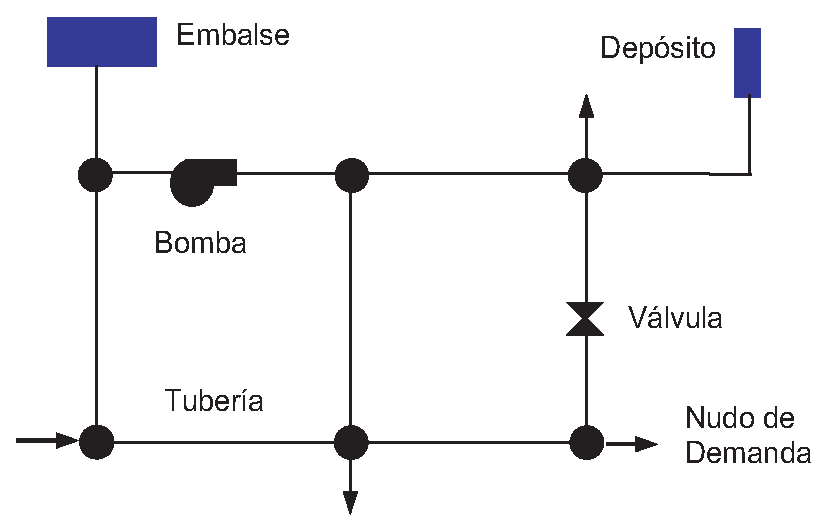
\includegraphics{Capitulo2/assets/componentesfisicosred.eps}
	\centering
	\caption[Componentes f�sicos de un sistema de distribuci�n de agua]{Componentes f�sicos de un sistema de distribuci�n de agua~\cite{Rossman2017}}
	\label{fig:componentesfisicos}
\end{figure}
\subsubsection{Componentes}
\paragraph{Nodos de consumo:} Son los puntos o extremos de una tuber�a, los cuales tambi�n permiten que estas se unan. Estos nudos pueden actuar como nudos de demanda a trav�s de los cuales el flujo abandona la red.

\paragraph{Reservorio:} Es una fuente de alimentaci�n externa. (Fuente de alimentaci�n externa desde la que se extrae el agua para alimentar la red, esta fuente puede ser un embalse, un rio, un lago, etc.)
\paragraph{Deposito:} Son elementos con la capacidad de almacenar agua.
\paragraph{Tuberias:} Es el medio por el cual transita el agua desde un lugar a otro.
\paragraph{Bombas:} Son el componente que permiten impulsar el liquido con el fin de elevarlo a una posici�n superior.
\paragraph{V�lvulas:} Elementos que limitan la presi�n o el caudal que transita en un punto de la red.